\documentclass[a4paper, 11pt, final, garamond]{book}
\usepackage{cours-preambule}

\makeatletter
\renewcommand{\@chapapp}{Thermodynamique -- chapitre}
\makeatother

\hfuzz=5.002pt

% \toggletrue{student}
% \toggletrue{corrige}
% \renewcommand{\mycol}{black}
\renewcommand{\mycol}{gray}

\begin{document}
\setcounter{chapter}{0}

\settype{enon}
\settype{solu_prof}
\settype{solu_stud}

\chapter{\cswitch{Correction du TD}{TD~: Systèmes thermodynamiques}}

\resetQ
\section{Pression des pneus}
\enonce{%
	La pression préconisée sur les roues avant d'une Mégane est de \SI{2.2}{bar}.
	On règle la pression des pneus un jour froid de cet hiver, par une température
	extérieure de $\SI{-5}{\degreeCelsius}$.
}%
\QR{%
	En supposant que le volume des pneus ne varie par et qu'il n'y a aucune fuite
	d'air possible, quelle sera l'indication du manomètre un jour chaud cet été,
	par une température extérieure de $\SI{30}{\degreeCelsius}$~?
}{%
	Comme la quantité de matière $n$ d'air contenue dans le pneu et son volume
	sont des constantes, alors d'après l'équation d'état du gaz parfait on a
	\begin{gather*}
		\frac{P_1}{T_1} = \frac{P_2}{T_2} = \frac{nR}{V}
		\\\Lra
		\boxed{P_2 = \frac{T_2}{T_1}P_1}
		\Ra
		\xul{P_2 = \SI{2.5}{bar}}
	\end{gather*}
}%
\QR{%
	Calculer la variation relative de pression due au changement de température.
	Que conseillez-vous~?
}{%
	La variation relative de pression est $\Delta{P}/P_1 = 14\%$. Elle est
	supérieure à 10\%, ce qui est loin d'être négligeable. Le meilleur conseil à
	donner est de refaire la pression des pneus~! Notez par ailleurs qu'il est
	préconisé de la vérifier chaque mois, et \textbf{indispensable} de le faire au
	moins deux fois par an \textbf{et} avant les grands trajets.
}%

\resetQ
\section{Fuite d'hélium}
\enonce{%
	On considère une bouteille de volume constant $V = \SI{10}{L}$ contenant de
	l'hélium, modélisé comme un gaz parfait monoatomique, à la pression $P =
		\SI{2.1}{bar}$ et à la température $T = \SI{300}{K}$.
	\begin{tcn}(data)<lfnt>{Données}
		$M(\ce{He}) = \SI{4.0}{g.mol^{-1}}$, $k_B = \SI{1.38e-23}{J.K^{-1}}$.
	\end{tcn}
}%
\QR{%
	Calculer la masse $m$ d'hélium dans la bouteille, puis la densité particulaire
	$n^*$, c'est-à-dire le nombre d'atomes par unité de volume.
}{%
	\noindent
	\begin{minipage}[t]{.25\linewidth}
		\begin{center}
			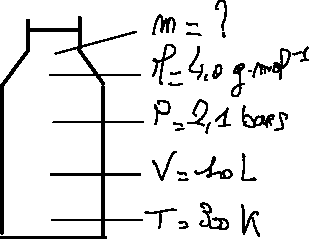
\includegraphics[width=\linewidth]{fuite_a}
		\end{center}
	\end{minipage}
	\hfill
	\begin{minipage}[t]{.73\linewidth}
		\begin{gather*}
			PV = nRT \qet m = nM
			\\\Lra
			\boxed{m = \frac{PVM}{RT}}
			\Lra
			\xul{
				m = \SI{3.4}{g}
			}
			\qav
			\left\{
			\begin{array}{rcl}
				P & = & \SI{2.1e5}{Pa}
				\\
				V & = & \SI{10e-3}{m^3}
				\\
				M & = & \SI{4.0e-3}{kg.mol^{-1}}
				\\
				R & = & \SI{8.314}{J.K^{-1}.mol^{-1}}
				\\
				T & = & \SI{300}{K}
			\end{array}
			\right.
		\end{gather*}
	\end{minipage}
	\begin{gather*}
		n^* = \frac{N}{V}
		\qqav
		N = n\Nc_A
		\qet
		n = \frac{m}{M}
		\Lra
		\boxed{n^* = \frac{m\Nc_A}{MV}}
		\qav
		\left\{
		\begin{array}{rcl}
			m     & = & \SI{3.4}{g}
			\\
			\Nc_A & = & \SI{6.022e23}{mol^{-1}}
			\\
			M     & = & \SI{4.0}{g.mol^{-1}}
			\\
			V     & = & \SI{10e-3}{m^{3}}
		\end{array}
		\right.\\
		\AN
		\xul{
			n^* = \SI{5.1e25}{m^{-3}}
		}
	\end{gather*}
}%
\QR{%
	Calculer la vitesse quadratique moyenne des atomes.
}{%
	\leavevmode\vspace*{-15pt}\relax
	\begin{gather*}
		\beforetext{Température cinétique $\Ra$}
		\frac{1}{2}m{v^*}^2 = \frac{3}{2}k_BT
		\qqav
		m = \frac{M}{\Nc_A}
		\qet
		R = \Nc_Ak_B
		\\\Lra
		\boxed{v^* = \frac{3RT}{M}}
		\Ra
		\xul{v^* = \SI{1.4e3}{m.s^{-1}}}
	\end{gather*}
}%
\QR{%
	À la suite de l'ouverture de la bouteille, la pression passe à $P' =
		\SI{1.4}{bar}$ et la température à $T' = \SI{290}{K}$. Calculer la masse
	$\Delta{m}$ de gaz qui s'est échappé de la bouteille.
}{%
	\noindent
	\begin{minipage}[t]{.25\linewidth}
		\begin{center}
			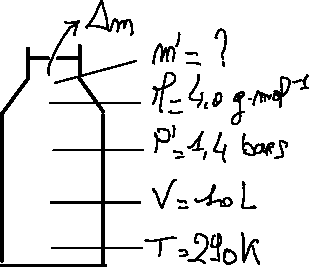
\includegraphics[width=\linewidth]{fuite_b}
		\end{center}
	\end{minipage}
	\hfill
	\begin{minipage}[t]{.73\linewidth}
		\begin{gather*}
			\boxed{m' = \frac{P'VM}{RT'}}
			\Ra
			\xul{
				m = \SI{2.0}{g}
			}
			\\
			\Delta{m} = m - m'
			\Lra
			\xul{\Delta{m} = \SI{1.0}{g}}
		\end{gather*}
	\end{minipage}
}%
\QR{%
	On a vite refermé la bouteille. À quelle température $T''$ faudrait-il porter
	le gaz pour atteindre à nouveau la pression $P$~? L'exprimer en fonction de
	$P$, $P'$ et $T'$.
}{%
	On garde $m'$ et $V$, on revient à $P'' = P$ et on cherche $T''$~:
	\[
		\boxed{T'' = \frac{PVM}{m'R} = \frac{P}{P'}T'}
		\Ra
		\xul{T'' = \SI{435}{K} = \SI{4.4e2}{K}}
	\]
}%

\resetQ
\section{Gaz parfait dans une enceinte}
\enonce{%
	Une quantité de matière $n$ de gaz parfait est enfermée dans une enceinte de
	surface de section $S$. Cette enceinte est fermée par un piston de masse $m$,
	à même de coulisser sans frottement, et permet les transferts thermiques, si
	bien que lorsqu’on attend suffisamment longtemps le gaz contenu dans
	l’enceinte est en équilibre thermique avec l’extérieur. Le milieu extérieur se
	trouve à température et pression constantes $T_0$ et $P_0$ . On fait subir au
	gaz la série de transformations suivante~:
	\begin{enumerate}[label=\clenumi]
		\item Initialement, dans l'état (1), le système est au repos depuis
		      suffisamment longtemps pour avoir atteint l'équilibre thermique et
		      mécanique~;
		\item État (2)~: le gaz est chauffé jusqu'à ce qu'il atteigne la température
		      $T > T_0$, on est à l'équilibre dynamique~;
		\item État (3)~: on place brusquement une masse supplémentaire $M$ sur le
		      piston, l'équilibre thermique n'est pas atteint~;
		\item État (4)~: l'équilibre thermique est atteint.
	\end{enumerate}
	\begin{center}
		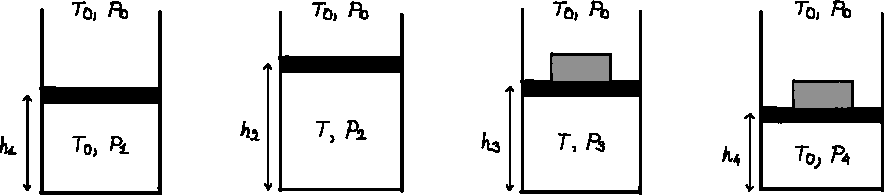
\includegraphics[width=.8\linewidth]{piston-plain}
	\end{center}
}%
\QR{%
	Exprimer les hauteurs $h_1$ à $h_4$ du piston dans chaque état, en fonction
	des grandeurs d'état d'abord, puis en fonction de $h_1$ ensuite.
}{%
	On trace les 4 situations~:
	\smallbreak
	\noindent
	\begin{minipage}[t]{.24\linewidth}
		\begin{center}
			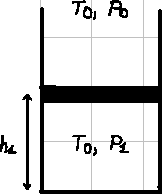
\includegraphics[height=4cm]{piston_1}
			\captionsetup{justification=centering}
			\captionof*{figure}{\vspace{-15pt}\\\circled{1}\\Équilibre
				thermodynamique\\$P_1 > P_0$}
		\end{center}
	\end{minipage}
	\hfill
	\begin{minipage}[t]{.24\linewidth}
		\begin{center}
			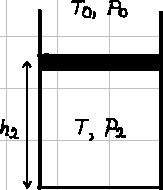
\includegraphics[height=4cm]{piston_2}
			\captionsetup{justification=centering}
			\captionof*{figure}{\vspace{-15pt}\\\circled{2}\\Équilibre dynamique\\$T >
				T_0~;~V_2>V_1~;~P_2>P_0$}
		\end{center}
	\end{minipage}
	\hfill
	\begin{minipage}[t]{.24\linewidth}
		\begin{center}
			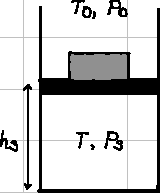
\includegraphics[height=4cm]{piston_3}
			\captionsetup{justification=centering}
			\captionof*{figure}{\vspace{-15pt}\\\circled{3}\\Équilibre
				dynamique\\$T~;~V_3<V_2~;~P_3>P_2$}
		\end{center}
	\end{minipage}
	\hfill
	\begin{minipage}[t]{.24\linewidth}
		\begin{center}
			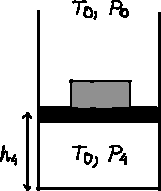
\includegraphics[height=4cm]{piston_4}
			\captionsetup{justification=centering}
			\captionof*{figure}{\vspace{-15pt}\\\circled{4}\\Équilibre
				thermodynamique\\$T=T_0~;~V_4<V_1~;~P_4>P_1$}
		\end{center}
	\end{minipage}
	\begin{enumerate}[label=\clenumi]
		\item
		      \begin{minipage}[t]{.70\linewidth}
			      \begin{itemize}
				      \bitem{Système}~: \{piston\}, référentiel laboratoire supposé
				      galiléen.
				      \bitem{Repère}~: cartésien, $z$ vertical ascendant~;
				      \textbf{repérage} $\OM = z \uz$.
				      \bitem{BdF}~:
				      \leavevmode\vspace*{-15pt}\relax
				      \[
					      \left\{
					      \begin{array}{rcl}
						      \Pf          & = & -mg\uz
						      \\
						      \Ff\ind{ext} & = & -P_0S \uz
						      \\
						      \Ff\ind{int} & = & P_1S\uz
					      \end{array}
					      \right.
				      \]
				      \bitem{Condition d'équilibre}~:
				      \begin{gather*}
					      \sum_i \Ff_i = \of
					      \Lra
					      (P_1-P_0)S = mg
					      \Lra
					      P_1S = P_0S + mg
					      \tag{1}
					      \label{eq:1}
				      \end{gather*}
			      \end{itemize}
		      \end{minipage}
		      \hfill
		      \begin{minipage}[t]{.20\linewidth}
			      \vspace{0pt}
			      \begin{center}
				      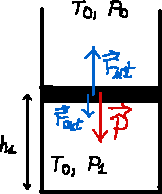
\includegraphics[width=\linewidth]{piston_forces}
			      \end{center}
		      \end{minipage}
		      \begin{itemize}
			      \item[]
				      \begin{gather*}
					      \beforetext{Gaz parfait~:}
					      P_1V_1 = nRT_0
					      \qet
					      V_1 = h_1S
					      \qdc
					      P_1h_1S = nRT_0
					      \\\Ra
					      h_1 P_1S = nRT_0
					      \tag{1'}
					      \label{eq:1p}
					      \\\Lra
					      \boxed{h_1 = \frac{nRT_0}{P_0S + mg}}
				      \end{gather*}
		      \end{itemize}
		\item Même système, mêmes forces avec $\Ff\ind{int} = P_2S\uz$ et $P_2h_2S =
			      nRT$, d'où
		      \begin{gather*}
			      P_2S = P_0S + mg = P_1S
			      \tag{2}
			      \label{eq:2}
			      \\\beforetext{et}
			      h_2 P_1S = nRT
			      \tag{2'}
			      \label{eq:2p}
			      \\\beforetext{d'où}
			      \boxed{h_2 = \frac{nRT}{P_0S + mg}}
			      \qet
			      \boxed{h_2 = h_1 \times \frac{T_0}{T}}
			      \qav
			      \eqref{eq:1p} \text{~et~} \eqref{eq:2p}
		      \end{gather*}
		\item Température inchangée, mais forces extérieures modifiées~: on passe de
		      $m$ à $m+M$, la pression intérieure doit compenser ces forces~:
		      \begin{gather*}
			      P_3S = P_0S + (m+M)g
			      \tag{3}
			      \label{eq:3}
			      \\\beforetext{et}
			      h_3 P_3S = nRT
			      \tag{3'}
			      \label{eq:3p}
			      \\\beforetext{d'où}
			      \boxed{h_3 = \frac{nRT}{P_0S + (m+M)g}}
			      \\\beforetext{avec~\eqref{eq:3p}~et~\eqref{eq:2p}}
			      \boxed{h_3 = h_2 \frac{P_1}{P_3}}
			      \tag{3''}
			      \label{eq:3s}
		      \end{gather*}
		      \begin{tcn}(ror){Transformations rapides}
			      Les équilibres thermiques sont plus lents à atteindre que les équilibres
			      mécaniques~: une variation mécanique brusque implique un potentiel
			      équilibre mécanique \textbf{avant} l'équilibre thermique.
		      \end{tcn}
		\item De même~:
		      \begin{gather*}
			      P_4S = P_0S + (m+M)g = P_3S
			      \tag{4}
			      \label{eq:4}
			      \\\beforetext{et}
			      h_4 P_4S = nRT_0
			      \tag{4'}
			      \label{eq:4p}
			      \\\beforetext{d'où}
			      \boxed{h_4 = \frac{nRT_0}{P_0S + (m+M)g}}
			      \\\beforetext{avec~\eqref{eq:4p}, \eqref{eq:1p}~et~\eqref{eq:3s}}
			      \boxed{h_4 = \frac{h_1h_3}{h_2}}
		      \end{gather*}
	\end{enumerate}
}%

\resetQ
\section{Ressort à gaz}
\enonce{%
	Les sièges de bureaux sont souvent montées sur un vérin cylindrique permettant
	d'en ajuster la hauteur. On décrit ce vérin cylindrique à air comprimé, supposé
	parfait, par le schéma ci-dessous.
	\begin{center}
		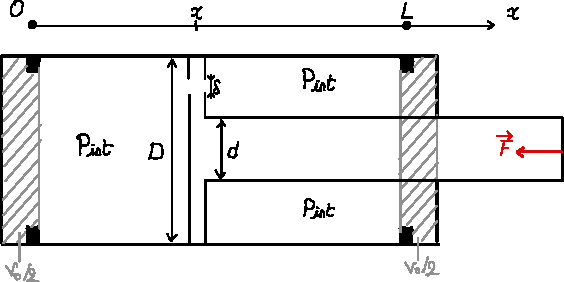
\includegraphics[width=.7\linewidth]{ressort_gaz-plain}
	\end{center}
	Le piston a une épaisseur nulle, et on pourra négliger la section de l'orifice
	de communication de diamètre $\delta $ devant les autres sections. On note $V_0$
	l'ensemble des deux volumes morts que le piston ne peut atteindre, situés en
	$x<0$ et $x>L$. On prendra également $D = 2d$. On supposera que l'équilibre
	thermique du gaz avec l'air extérieur de température $T_0$ est réalisé pour
	toute position du piston, et on note $P_0$ la pression extérieure.
}%
\QR{%
	Exprimer le volume $V(x)$ disponible pour le gaz dans le vérin en fonction de
	$L$, $x$ et $d$.
}{%
	\noindent
	\begin{minipage}[t]{.70\linewidth}
		On somme le volume de gauche, celui du cylindre de hauteur $x$ et celui du
		cylindre de longueur $L-x$ qui est occupé par le piston, sans oublier les
		volumes morts et sachant que $D = 2d$~:
		\begin{align*}
			V(x)         & = V_0 + x\pi d^2 + (L-x) \left( \pi d^2 - \pi \frac{d^2}{4} \right)
			\\\Lra
			\Aboxed{V(x) & = V_0 + \frac{\pi d^2}{4} (x+3L)}
		\end{align*}
	\end{minipage}
	\hfill
	\begin{minipage}[t]{.25\linewidth}
		\vspace{0pt}
		\begin{center}
			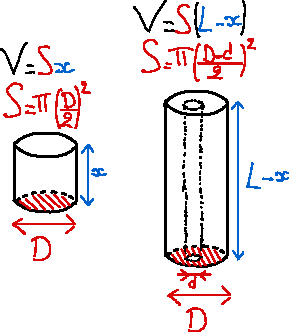
\includegraphics[width=\linewidth]{ressort_gaz-volu}
		\end{center}
	\end{minipage}
}%
\QR{%
	Donnez l'expression de $p\ind{int}(x)$ en fonction de $V(x)$.
}{%
	On a un gaz parfait~:
	\[
		\boxed{P\ind{int}(x) = \frac{nRT_0}{V(x)}}
	\]
}%
\QR{%
	On suppose le système à l'équilibre mécanique avec le piston à la position
	$x$. Une personne s'assoie sur le siège, exerçant une force $\Ff$. Exprimer la
	force $\Ff'$ qu'exerce la tige sur le système extérieur.
}{%
	\noindent
	\begin{minipage}[t]{.50\linewidth}
		\begin{itemize}
			\bitem{Système} = \{piston + tige\}
			\bitem{BdF}~:
			\leavevmode\vspace*{-15pt}\relax
			\[
				\left\{
				\begin{array}{rcl}
					\Ff\ind{air,g}   & = & P\ind{int}(x) (\pi d^2)\ux
					\\
					\Ff\ind{air,d}   & = & -P\ind{int}(x) (\pi \frac{d^4}{4})\ux
					\\
					\Ff\ind{air,ext} & = & - P_0\pi \frac{d^2}{4}\ux
					\\
					\Ff
				\end{array}
				\right.
			\]
		\end{itemize}
	\end{minipage}
	\hfill
	\begin{minipage}[t]{.45\linewidth}
		\vspace{0pt}
		\begin{center}
			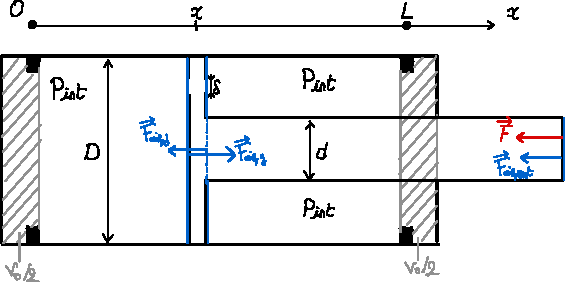
\includegraphics[width=\linewidth]{ressort_gaz-forces}
		\end{center}
	\end{minipage}
	\begin{itemize}
		\bitem{Condition d'équilibre}~: on cherche $\Ff' = -\Ff$, avec
		\begin{gather*}
			\Ff\ind{air,g} + \Ff\ind{air,d} + \Ff\ind{air,ext} + \Ff = \of
			\\\Lra
			\beforetext{sur $\ux$}
			\Ff = \frac{\pi d^2}{4} \left( (4-1)P\ind{int}(x) - P_0 \right)
			\\\Lra
			\boxed{\Ff = \frac{\pi d^2}{4} (3P\ind{int} - P_0)}
		\end{gather*}
	\end{itemize}
}%

\resetQ
\section{Recherche d'un état final}
\enonce{%
	\noindent
	\begin{minipage}[c]{.65\linewidth}
		Une enceinte indéformable aux parois calorifugées\ftn{Qui ne laisse pas passer la
			chaleur.} est séparée en deux compartiments par une cloison étanche de surface
		$S$, mobile, diathermane\ftn{Qui laisse passer la chaleur.} et reliée à un
		ressort de constante de raideur $k$. Les deux compartiments contiennent chacun
		un gaz parfait. Dans l’état initial, le gaz du compartiment 1 est dans l’état
		($T_0$, $V_0$, $P_0$, $n$), le gaz du compartiment 2 dans l’état ($T_0$, $V_0$,
		$2P_0$, $2n$), une cale bloque la cloison mobile et la longueur du ressort est
		égale à sa longueur à vide. On enlève la cale et on laisse le système atteindre
		un état d’équilibre.
	\end{minipage}
	\hfill
	\begin{minipage}[c]{.33\linewidth}
		\vspace{0pt}
		\begin{center}
			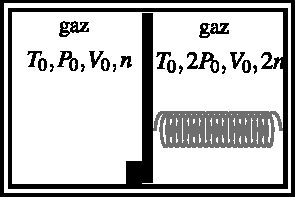
\includegraphics[width=\linewidth]{etat_fin-plain}
		\end{center}
	\end{minipage}
}%
\QR{%
	Décrire qualitativement l'évolution du système.
}{%
	Initialement, $P\ind{droite} > P\ind{gauche}$, donc la paroi est poussée vers
	la gauche. Elle suivra ensuite des oscillations amorties.
}%
\QR{%
	Écrire cinq relations faisant intervenir certaines des six variables d'état~:
	$V_1$ et $V_2$ les volumes finaux de chaque compartiment, $P_1$ et $P_2$ leurs
	pressions, et $T_1$ et $T_2$ leurs températures.
}{%
	On a~:
	\begin{enumerate}
		\item Conservation du volume total~: $2V_0 = V_1+V_2$
		\item GP compartiment 1~:
		      \begin{gather*}
			      P_0V_0 = nRT_0
			      \qMath{puis}
			      P_1V_1 = nRT_1
			      \qdc
			      \frac{P_0V_0}{T_0} = \frac{P_1V_1}{T_1}
		      \end{gather*}
		\item GP compartiment 2~:
		      \begin{gather*}
			      2P_0V_0 = 2nRT_0
			      \qMath{puis}
			      P_2V_2 = 2nRT_2
			      \qdc
			      \frac{2P_0V_0}{T_0} = \frac{P_2V_2}{T_2}
		      \end{gather*}
		\item Équilibre thermique à la fin~: $T_1=T_2$
		\item Équilibre mécanique sur la paroi. Avec $\Ff = +k (x_2-x_0)\ux$ la force
		      de rappel du ressort, $x_2 = V_2/S$ et $x_0 = V_0/S$. Avec les forces de
		      pressions, on obtient
		      \begin{align*}
			      P_1S - P_2S + k \frac{V_2 - V_0}{S} & = 0
			      \\\Lra
			      P_2                                 & = P_1 + k \frac{V_2-V_0}{S^2}
		      \end{align*}
	\end{enumerate}
	\begin{tcn}(impo){Parois diathermanes, calorifugées}
		\begin{itemize}
			\item Parois \textbf{diathermanes} signifie qui \textbf{laisse passer la
				      chaleur}~;
			\item Paroi externes calorifugées $\Ra$ pas de transfert thermique
			      \textbf{à l'extérieur}~: a priori, $T_1 = T_2 \boxed{\neq} T_0$~! On
			      trouvera avec le premier principe que
			      \[
				      T_1 = T_0 - \frac{k}{6nC_v} \left( \frac{V_2-V_0}{S} \right)^2
				      \qso
				      \boxed{T_1 < T_0}
			      \]
		\end{itemize}
	\end{tcn}
}%

\end{document}
